\section{Introduction}

This is a specification for the Spam protocol. Its a point-to-point packet protocol, which will be used by the device to communicate the status of on-going tests to a host. The host would in-turn use this to visually indicate the test status to the operator. It uses the EzLink protocol for communication. You can think of the Spam protocol as an application layer specification .

\section{Packet}

Every packet consists of 3 parts; the EzLink  header, followed by the application header, and the actual payload. \\

\begin{bytefield}[bitwidth=1.1em]{32}
\bitbox{8}{EzLink Header} &
\bitbox{8}{Spam Header} &
\bitbox{8}{Payload...} \\
\end{bytefield}

For more information on EzLink see the following:

\textless rdar://problem/16541301\textgreater  'EzLink' host-library

\textless rdar://problem/16541321\textgreater  'EzLink' diags-side library

\section{Goals}

The primary goal of this protocol is to send status updates from the device to the host. The device in this case is the unit that is undergoing testing, traditionally known as DUT(Device Under Test). The host could be a computer, or even a micro-controller on the cable that is snooping data being sent from the DUT.

\subsection{Device Goals}

\begin{enumerate}
 \item Signal start of communication using the EzLinkSetup API.
 \item  Send a configuration packet that establishes the heartbeat interval `h' seconds.
 \item Send a status packet every `h' seconds.
\end{enumerate}

\subsection{Host Goals}

\begin{enumerate}
\item Parse the status packet and give an indication to the operator about the device state.
\item In case of an unresponsive device, give an indication to the operator. A device is deemed unresponsive(hung/panicked etc.) if the host has not received any packet for more than `$2\times h$' seconds.
\item If a packet is not supported ignore it without giving erring out. Even if the packet is unsupported this still counts towards refreshing the heartbeat. 
\end{enumerate}

%\newpage
\section{Communication}
The communication is always initiated by the device; all that the host does is send Acks back to the device. The sequence diagram is shown below.\\

%%%%%%%%%%%%%%%%%%%%%%%%%%%%%%%%% 
%           Communication Sequence Diagram                               %
%%%%%%%%%%%%%%%%%%%%%%%%%%%%%%%%%

\begin{figure}[H]
\caption{SPAM Communication Sequence}
% Agents
\def\Device{Device}
\def\Host{Host}

% Flows
\def\Req{Req}
\def\Ack{Ack}

% Diagram
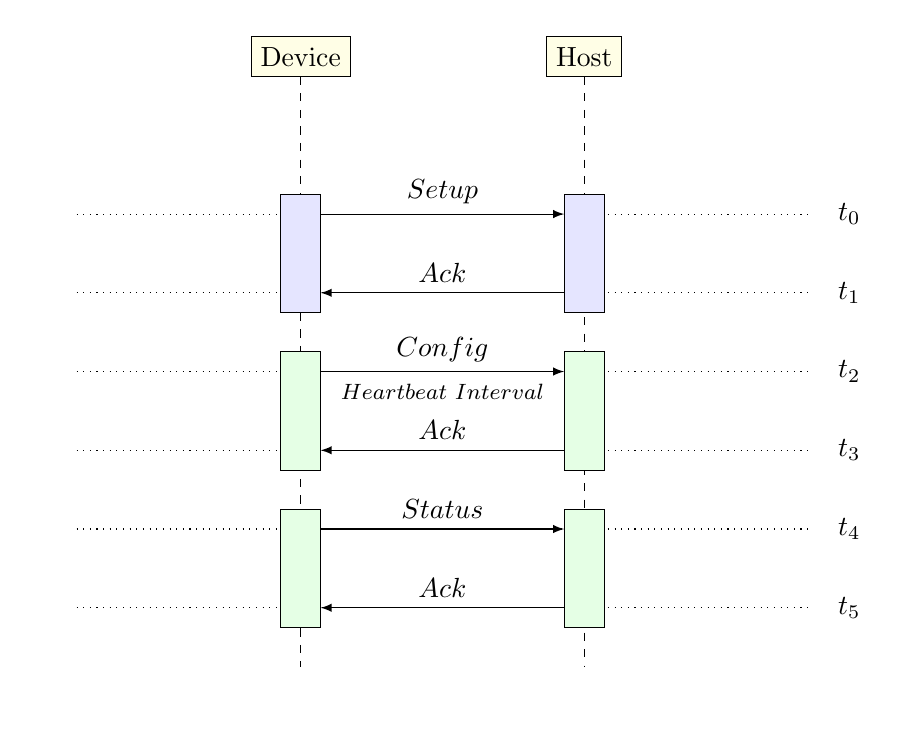
\begin{tikzpicture}[every node/.style={font=\normalsize,
  minimum height=0.5cm,minimum width=0.5cm},]

% Matrix
\node [matrix, very thin,column sep=1.3cm,row sep=0.5cm] (matrix) at (0,0) {
 
&&\node(0,0) (\Device) {};
&&\node(0,0) (\Host) {};\\ 
  
&&\node(0,0) (\Device 0) {};
&&\node(0,0) (\Host 0) {};\\ 

\node(0,0) (t0 left) {};
&&\node(0,0) (\Device 1) {};
&\node(0,0) (\Req 1) {};
&\node(0,0) (\Host 1) {};
&&\node(0,0) (t0 right) {};\\

\node(0,0) (t1 left) {};
&&\node(0,0) (\Device 2) {};
&\node(0,0) (\Ack 1) {};
&\node(0,0) (\Host 2) {};
&&\node(0,0) (t1 right) {};\\
 
\node(0,0) (t2 left) {}; 
&&\node(0,0) (\Device 3) {};
&\node(0,0) (\Req 2) {};
&\node(0,0) (\Host 3) {};
&&\node(0,0) (t2 right) {};\\

\node(0,0) (t3 left) {}; 
&&\node(0,0) (\Device 4) {};
&\node(0,0) (\Ack 2) {};
&\node(0,0) (\Host 4) {};
&&\node(0,0) (t3 right) {};\\

\node(0,0) (t4 left) {}; 
&&\node(0,0) (\Device 5) {};
&\node(0,0) (\Req 3) {};
&\node(0,0) (\Host 5) {};
&&\node(0,0) (t4 right) {};\\

\node(0,0) (t5 left) {}; 
&&\node(0,0) (\Device 6) {};
&\node(0,0) (\Ack 3) {};
&\node(0,0) (\Host 6) {};
&&\node(0,0) (t5 right) {};\\

&&\node(0,0) (\Device 7) {};
&&\node(0,0) (\Host 7) {};\\ 
};

% Agents labels
\fill 
	(\Device) node[draw,fill=yellow!10] {\Device}
	(\Host) node[draw,fill=yellow!10] {\Host};

% Horizontal time lines
\draw [dotted] 
  (t0 left) -- (t0 right) node[right] {$t_{0}$}
  (t1 left) -- (t1 right) node[right] {$t_{1}$}
  (t2 left) -- (t2 right) node[right] {$t_{2}$}
  (t3 left) -- (t3 right) node[right] {$t_{3}$}
  (t4 left) -- (t4 right) node[right] {$t_{4}$}
  (t5 left) -- (t5 right) node[right] {$t_{5}$};

% Vertical timeline
\draw [dashed] 
  (\Device) -- (\Device 1) (\Device 2) -- (\Device 7)
  (\Host) -- (\Host 1) (\Host 1) -- (\Host 7);


% Vertical flows (timeline)
%\draw [-latex] (\Host 4) -- (\Host 5);

% Blocks (Xaction)
\filldraw[fill=blue!10]
  (\Host 1.north west) rectangle (\Host 2.south east)
  (\Device 1.north west) rectangle (\Device 2.south east);
  
\filldraw[fill=green!10]
  (\Host 3.north west) rectangle (\Host 4.south east)
  (\Device 3.north west) rectangle (\Device 4.south east);
 
\filldraw[fill=green!10]
  (\Host 5.north west) rectangle (\Host 6.south east)
  (\Device 5.north west) rectangle (\Device 6.south east);

% Horizontal flows (Packet Xfers)
\draw [-latex] (\Device 1) -- (\Host 1);
\draw [-latex] (\Host 2) -- (\Device 2);
\draw [-latex] (\Device 3) -- (\Host 3);
\draw [-latex] (\Host 4) -- (\Device 4);
\draw [-latex] (\Device 5) -- (\Host 5);
\draw [-latex] (\Host 6) -- (\Device 6);


% Flows Labels 
\fill
  (\Req 1) 
    node[above] {$Setup$}
  (\Ack 1) 
    node[above] {$Ack$}
  (\Req 2)
  	node[above] {$Config$}
    node[font=\footnotesize, below] {$Heartbeat\ Interval$}
  (\Ack 2) 
    node[above] {$Ack$}
  (\Req 3)
  	node[above] {$Status$}
  (\Ack 3) 
    node[above] {$Ack$};

\end{tikzpicture}
\end{figure}
%%%%%%%%%%%%%%%%%%%%%%%%%%%%%%%%% 

\subsection{Setup}
This is used by the device to discover the host and make sure its responsive. If this fails, the device will not initiate the Spam protocol

\subsection{Configure}
In this phase the device will setup the heartbeat interval. In between the setup and configure phases the host can assume a default heartbeat timeout that is sufficiently long ( say 2min ). Once the configure packet is received the host will update it's heartbeat timeout. The device can send configure packets at any point. For example if the host knows that it is going to be doing something during which time it might not be able to send packets to the host ( one of the scenarios is when the device boots from EFI to OS ), it can send a configure packet with a sufficiently long heartbeat interval.

\subsection{Status Reporting}
This is used by the device to report it's status to the host. To make implementation simple, since we know that the host in our case is going to control 3 LEDs we can have the packet contents directly control the LEDs. The plan is to add additional packet types later on.

\section{Spam Packet Structure}

\subsection{Header}

\floatstyle{plain}
\restylefloat{figure}

\begin{figure}[htbp]
  \centering
  \begin{bytefield}{32}
    \bitheader{0,7-8,15-16,23-24,31} \\
      % We have to do the \parbox explicitly in the next line because
      % \hyperlink typesets its argument in horizontal mode.
      \bitbox{16}{\hyperlink{spam-version}{\parbox{\width}{\centering Version}}} &
      \bitbox{16}{\hyperlink{packet-type}{Type}} \\
      \bitbox{32}{\hyperlink{packet-length}{Length}} \\
  \end{bytefield}
  \caption{Spam Header}
  \label{fig:spam-hdr}
\end{figure}

\hypertarget{spam-version}{\subsubsection{Version}}
   The first 16 bits of the packet are the Spam protocol version number. This document describes version 1 of the Spam Protocol and thus the version field has a value of 0x01.

\hypertarget{packet-type}{\subsubsection{Type}}
  This field is used to identify the types of packets. The possible values for this are:
  
\begin{center}
\renewcommand{\arraystretch}{1.5}
\begin{longtable}{llp{0.6\textwidth}}
   Type & Description \\ \hline
   0x0  & Configure Packet \\
   0x1  & LED Control Packet \\
   0x2 &  Heartbeat Packet \\
\end{longtable}
\end{center}

\hypertarget{packet-length}{\subsubsection{Length}}
  This indicates the size of the payload, not including the size of the Spam Header itself. 
  
\subsection{Configure Packet}

The configure packet payload will be nothing but a 32bit value that indicates the heartbeat interval in seconds

\begin{figure}[htbp]
  \centering
  \begin{bytefield}{32}
    \bitheader{0,31} \\
      \wordbox{1}{Heartbeat Interval}\\
  \end{bytefield}
  \caption{Configure}
  \label{fig:spam-cfg}
\end{figure}

\subsection{LED Control Packet}

This will be used by the device to control the LEDs on the host side. 

\begin{figure}[htbp]
  \centering
  \begin{bytefield}[bitwidth=1.1em]{24}
    \bitheader{0,7-8,15-16,23} \\
      \bitbox{8}{Red LED}& 
      \bitbox{8}{Green LED}&
      \bitbox{8}{Yellow LED}\\
      \bitbox{8}{IsFinished LED}&
      \bitbox{8}{TempAlert LED}\\
  \end{bytefield}
  \caption{LED Control}
  \label{fig:spam-cfg}
\end{figure}

Each LED can be controlled by it's corresponding 8bit value.

\begin{center}
\renewcommand{\arraystretch}{1.5}
\begin{longtable}{llp{0.6\textwidth}}
   Value & Description \\ \hline
   0x0  & Off \\
   0x1  & On \\
   0x2  & Slow Pulse(every 3s) \\
   0x3 & Fast Pulse(every 0.5s)
\end{longtable}
\end{center}

\subsection{Heartbeat Packet}

This packet type has no payload. The 'Length' field for this packet should be set to 0. The Device is responsible for sending a heartbeat packet at the frequency dictated by the heartbeat interval.

\section{LED Behavior}

The Device is essentially in control of what packets it sends over to the Host, and hence controls which LEDs are lit up ( there are some exceptions to this rule that will be highlighted below ) The various LED states are as follows

\begin{enumerate}
\item {\bfseries Plugged In}: The device has not yet sent the Setup packet. To indicate this the Host should set the Yellow LED to 'Slow Pulse' and all other LEDs to 'Off'.
\item {\bfseries Ongoing}:  Indicates that a test is in progress. We should set the Yellow LED to 'On', and all other LEDs to 'Off'.
\item {\bfseries  Pass}: Indicates that test has successfully finished. We should set Green LED and IsFinished LED to 'On'; all other LEDs should be 'Off'.
\item {\bfseries Fail}: Indicates that test has failed. We should set Red LED and IsFinished to 'On'; all other LEDs should be 'Off'.
\item {\bfseries Unresponsive}: In this scenario, the Host's Heartbeat / Setup Timer has expired and it should set Red LED to 'Fast Pulse' and IsFinished LED to 'On'.
\item {\bfseries Temperature Alert}: The 'TempAlert' LED status indicates whether the temperature of the Device has gone above a maximum threshhold.
\end{enumerate}

%\newpage
\section{Host State Machine}

This describes the host side state machine that drives the LEDs

%%%%%%%%%%%%%%%%%%%%%%%%%%%%%%%%% 
%          Host State Machine                                                          %
%%%%%%%%%%%%%%%%%%%%%%%%%%%%%%%%%

\begin{figure}[H]
\caption{Host State Machine}
\begin{tikzpicture}[>=latex]

  %
  % Styles for states, and state edges
  %
  \tikzstyle{state} = [draw, very thick, fill=white, circle, minimum height=3em, minimum width=7em, node distance=8em, font={\sffamily\bfseries}]
  \tikzstyle{stateEdgePortion} = [black,thick];
  \tikzstyle{stateEdge} = [stateEdgePortion,->];
  \tikzstyle{edgeLabel} = [pos=0.5, text centered, font={\sffamily\small}];

  %
  % Position States
  %
  \node[initial, state, name=not_conn] {NOT\_CONN};
  \node[state, name=conn, below of=not_conn, xshift=8em] {CONN};
  \node[state, name=running, below of=not_conn, xshift=-8em] {RUN};
  \node[state, name=panic, below of=not_conn, yshift=-8em] {?};

  %
  % Connect States via edges
  %
  \path
 	(not_conn.east)	edge[stateEdge, bend right=15] node[edgeLabel, xshift=-1.5em, yshift=-1em]{Plugged In}	(conn.north)
    (conn.north)	edge[stateEdge, bend right=15] node[edgeLabel, xshift=2.4em]{Unplugged}				    (not_conn.east)
  	(conn.west)	edge[stateEdge] node[edgeLabel, xshift=-1.5em, yshift=0.5em]{Setup} 					    (running.east)
	(conn.south) 	edge[stateEdge, bend left=15] node[edgeLabel, xshift=3.5em]{Setup Timeout} 			    (panic.east)
	(running.north)	edge[stateEdge, bend left=15] node[edgeLabel, xshift=-2.4em]{Unplugged}				    (not_conn.west)
	(running.south)	edge[stateEdge, bend right=15] node[edgeLabel, xshift=-4.3em]{Heartbeat Timeout} 		(panic.west)
  	(running) 		edge[stateEdge, loop left] node[edgeLabel]{Packet}								        (running)
	(panic.north)	edge[stateEdge, bend right=15] node[edgeLabel, xshift=2em, yshift=-2em]{Unplugged}		(not_conn.south)
	(panic.west)	edge[stateEdge, bend right=15] node[edgeLabel, xshift=1.5em]{Setup}				        (running.south);
\end{tikzpicture}
\end{figure}

\begin{enumerate}
\item  '?' represents the Device that has paniced or has become unresponsive. 
\item The 'Heartbeat timeout' is dictated by the Config packet sent by the Device.
\item  The 'Setup Timeout' is useful to catch issues where the Device was connected to the Host but for some reason did not issue a Setup packet. This timeout should be 5min, which gives the Device more than enough time to boot into the OS and send a Setup packet.
\item If the Host receives a Setup packet in the '?' state, it should go to the 'RUN' state and set LEDs to represent \emph{'Ongoing'}.
\end{enumerate}

%\newpage
\section{Device State Machine}

This defines the Device side behavior.

%%%%%%%%%%%%%%%%%%%%%%%%%%%%%%%%% 
%          Device State Machine                                                       %
%%%%%%%%%%%%%%%%%%%%%%%%%%%%%%%%%
\begin{figure}[H]
\caption{Device State Machine}
\begin{tikzpicture}[>=latex]

%
% Styles for states, and state edges
 %
\tikzstyle{state} = [draw, very thick, fill=white, circle, minimum height=3em, minimum width=7em, node distance=8em, font={\sffamily\bfseries}]
\tikzstyle{stateEdgePortion} = [black,thick];
\tikzstyle{stateEdge} = [stateEdgePortion,->];
\tikzstyle{edgeLabel} = [pos=0.5, text centered, font={\sffamily\small}];

%
% Position States
%
\node[initial, state, name=not_conn] {NOT\_CONN};
\node[state, name=conn, right of=not_conn, xshift=8em] {CONN};

 %
 % Connect States via edges
 %

 \path
	(not_conn.north)    edge[stateEdge, bend left=40]	node[edgeLabel, color=green!50!black, yshift=-1em]{Setup}							        (conn.north)
    (conn.south)		edge[stateEdge, bend left=40]	node[edgeLabel, color=red!50!black, yshift=-0.75em]{Packet}							        (not_conn.south)
	(not_conn)			edge[stateEdge, loop right] 	node[edgeLabel, color=red!50!black, yshift=-2em, xshift=-2em]{Setup$_{Periodic}$}			(not_conn)
	(conn)			    edge[stateEdge, loop right] 	node[edgeLabel, color=green!50!black, yshift=-2em, xshift=-2em]{Heartbeat$_{Periodic}$}	    (conn)
	(conn)			    edge[stateEdge, loop below] 	node[edgeLabel, color=green!50!black, yshift=-0.5em]{Packet}				                (conn);

\end{tikzpicture}
\end{figure}

\begin{enumerate} 
\item Edges with 'green' labels indicate that the Device got an 'Ack' from the Host.
\item Edges with 'red' labels indicate that the Device failed to get an 'Ack' from the Host.
\item In the 'NOT\_CONN' state the Device will keep sending periodic Setup packet until it finally gets an 'Ack' from the Host at which point it transistions to the 'CONN' state.
\item In the 'CONN' state the Device is supposed to periodically send the 'Heartbeat' packet as an 'I am alive' signal to the Host.
\item If the Device fails to get an 'Ack' for any packet that it sends to the Host, it transitions back to the 'NOT\_CONN' state.
\end{enumerate}

